% 
%  chapter4.tex
%
\chapter{Architecture}\label{ch:architecture}
In this chapter we take a look at the architecture developed in the scope of CASCIFFO.
The chapter is structured as follows:
\begin{itemize}
    \item Global architecture - describes the architecture in a global manner;
    \item Data Model - presents the conceptual representation of the data structures that the application uses, and it defines how data is organized and related within the application;
    \item \acrlong{be} architecture - describes the architecture of the \acrlong{be} module;
    \item \acrlong{fe} architecture - describes the architecture of the \acrlong{fe} module.
\end{itemize}


\section{Global architecture}
The initial approach taken towards CASCIFFO was made following the monolithic architecture. A monolithic architecture consists in the development of software components within a single codebase. From an operating system's point of view, these components operate within one single application. The advantages brought by this design are centered around simplicity, the application is easier to deploy, test, debug and monitor. 
Applying this concept into context, the components developed were divided into three layers, the \acrshort{ui}, domain and data access layer. The first layer - data access layer - contains the data created and manipulated by the platform CASCIFFO; the second layer - domain layer - responsible for security and business processes within the platform; lastly the \acrshort{ui} layer corresponds to the presentation and logic of the user interface where user interaction begins.

The \acrlong{be} and \acrlong{fe} modules have distinct responsibilities within these layers, while the \acrshort{fe} contains all of the \acrshort{ui} layer, the \acrshort{be} consists of both domain and data access layer, as illustrated by~\ref{fig:layer-arch}. Finally, in addition to these layers, there's also a component inherent, although external, to the data access layer, the data base component, which is where all the data is stored.

\begin{figure}[H]
    \centering
    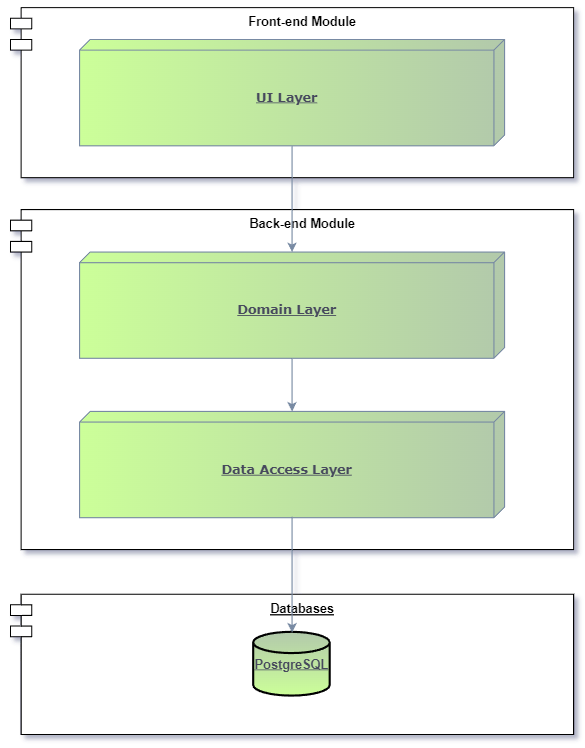
\includegraphics[scale=0.5]{Chapters/img/architecture/arch-layers.png}
    \caption{Layer Architecture}
    \label{fig:layer-arch}
\end{figure}

One of the drawbacks of this architecture is scalability and maintenance; the need of redeploying the entire application when a change is made, for example, a change in the \acrlong{fe} module should not imply an redeployment of the \acrlong{be} module as well. 
In wake of this, since we want a scalable solution, the layer based architecture was maintained while the monolithic aspect of a single codebase was discarded.
The modules were separated, allowing the \acrlong{fe} module and \acrlong{be} module to run independently of each other. Following the segregation of the modules, we also achieve independent deployments.

\section{Data model}


\section{\acrlong{be} module}

\section{\acrlong{fe} module}

\section{Deployment Architecture}
meter o apache ao barulho